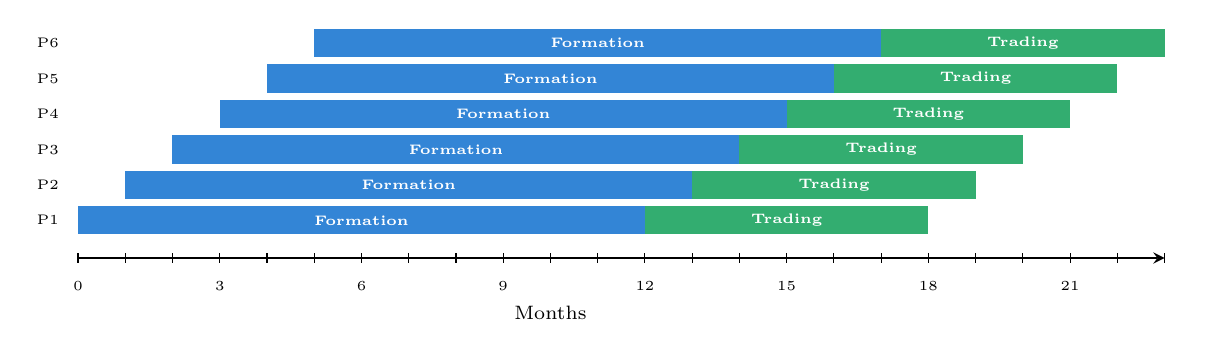
\begin{tikzpicture}[scale=0.6, font=\footnotesize]
  % Define colors
  \definecolor{formationcolor}{RGB}{0, 102, 204}
  \definecolor{tradingcolor}{RGB}{0, 153, 76}
  
  % Draw timeline axis
  \draw[thick, ->, >=stealth] (0,0) -- (23,0) node[right] {};
  
  % Draw month markers
  \foreach \x in {0,1,...,23} {
    \draw (\x,-0.1) -- (\x,0.1);
  }
  
  % Month labels
  \foreach \x/\label in {0/0,3/3,6/6,9/9,12/12,15/15,18/18, 21/21} {
    \node[below] at (\x,-0.3) {\tiny \label};
  }
  
  % Portfolio heights
  \def\pheight{0.6}
  \def\pgap{0.15}
  
  % Draw 6 portfolios
  \foreach \i in {1,...,6} {
    \pgfmathsetmacro\ystart{(\i-1)*(\pheight+\pgap)+0.5}
    \pgfmathsetmacro\xstart{\i-1}
    
    % Formation window
    \fill[formationcolor, opacity=0.8] (\xstart,\ystart) rectangle (\xstart+12,\ystart+\pheight);
    \node[white, font=\tiny\bfseries] at (\xstart+6,\ystart+\pheight/2) {Formation};
    
    % Trading window
    \fill[tradingcolor, opacity=0.8] (\xstart+12,\ystart) rectangle (\xstart+18,\ystart+\pheight);
    \node[white, font=\tiny\bfseries] at (\xstart+15,\ystart+\pheight/2) {Trading};
    
    % Labels
    \node[left] at (-0.2,\ystart+\pheight/2) {\tiny P\i};
  }
  
  % Month label
  \node[below] at (10,-0.8) {\scriptsize Months};
  
\end{tikzpicture}
